\chapter{Proponowane rozwiązanie}
W celu rozpoznania przechodnia został użyty połączony obraz termowizyjny i kolorowy. Następnie ten obraz zostaje poddany analizie HOG oraz klasyfikacji za pomocą SVM. W celu ustalenia obszaru zainteresowania na obrazie termowizyjnym za pomocą wzorca probabilistycznego zostają wytypowani kandydaci.

\section{Akwizycja obrazu}
Obraz kolorowy służy jako obraz bazowy. Rozdzielczości 640 x 480 pikseli, prędkością 30 klatek na sekundę i głębi 8 bitów na kanał. Źródłem tego obrazu jest kamera podłączona do układu za pomocą interfejsu HDMI. Na obraz bazowy zostaje nałożony obraz termowizyjny z kamery Lepton, który różni się znacząco parametrami. Abu je zsynchronizować zastosowano bufor ramki, do którego jest zapisywany obraz z prędkością 9 klatek na sekundę a odczytywany z prędkością 30. Kolejnym przekształceniem jest transformacja projekcyjna. Ma na celu powiększenie i dopasowanie obrazu by poprawnie pokrywał się z obraz wizyjnym. W tym celu został zaimplementowany moduł który oblicza na podstawie parametrów macierzy transformaty i koordynatami piksela obrazu źródłowego odpowiadającą mu pozycję na obrazie termowizyjnym zapisanym w buforze ramki. Następny moduł dokonuje interpolacji dwuliniowej. Do poprawnej interpolacji wymagane są 4 piksele otaczające obliczony z projekcji punkt. W celu zredukowania liczby dostępów do pamięci i zwiększenie szybkość działania moduł zapamiętuje 4 ostatnio użyte wartości pikseli. Rozwiązanie to pozwala na pracę w czasie rzeczywistym małym kosztem zasobów układu.
Strumień wizyjny jak i termowizyjny działają w AXI-Stream. Umożliwia to łatwą synchronizację obu obrazów na podstawie sygnału SOF (ang. Start o frame). Moduł synchronizacji czeka na pojawienie się tego sygnału w strumieniu termowizyjnym. Do tego momentu wszystkie napływające piksele są odrzucane. Gdy pojawi się sygnał strumień IR zostaje zatrzymany i czeka na pojawienie się sygnału SOF w bazowym strumieniu wizyjnym. Po jego wykryciu strumień IR rusza. Oba strumienie zostają zsynchronizowane tworząc strumień wizyjna obrazu RGBIR. Następnie ten strumień zostaje przesłany do pamięci za pośrednictwem VDMA oraz (po koloryzacji i nałożeniu) wyświetlony na monitorze przez port VGA.

\section{Wyznaczanie ROI}
Strumień IR z kamery zostaje zbinearyzowany i zbadany w detektorze DPM. Moduł DPM przesyła do pamięci listę koordynatów kandydatów wraz z mocą dopasowania. Moduł DPM został zaczerpnięty z pracy inżynierskiej. Moduł wykorzystuję strumień bezpośrednio z kamery. Wielkość okna detekcji wynosi 16 x 40 pikseli. Jeżeli badany obraz binarny wykazał odpowiedni poziom dopasowania do wzorca zostaje wysłana o tym informacja poprzez AXI-Stream do pamięci. Informacja zawiera koordynaty okna w układzie odniesienia kamery IR oraz wartość mocy dopasowania. Gdy zostanie zbadane ostatnie okno w obrazie zostaje wysłany sygnał LAST co wygeneruje przerwanie dla systemu procesorowego.

\section{Klasyfikacja za pomcą SVM}
Z lisy kandydatów wygenerowanej przez moduł DPM wybierany jest wynik o najwyższej mocy dopasowania. Koordynaty z układu odniesienia kamery zostają poddane transformacie projekcyjnej do układu odniesienia kamery RGB. Z obszaru na obrazie RGBIR zawierającym potencjalnie człowieka zostają wyodrębnione cechy HOG które następnie służą jako wektor dla SVM.

\section{Prezentacja wyników}
Na wyjściu konsoli zostają podane współrzędne oraz moc dopasowania i klasyfikacja obiektu. Na obrazie wyjściowym VGA obszar ten zostaje zaznaczony zieloną ramką. Jeżeli potencjalny obszar nie został zakwalifikowany jako człowiek ale miał największą moc dopasowania DPM to obszar zostaję zaznaczony czerwoną ramką. Czarna ramka oznacza że nie został wykryty żaden obiekt. 

\chapter{Implementacja}
\label{cha:impl}
\section{Sprzęt}
\subsection{Kamera termowizyjna Lepton} 
Lepton jest zintegrowaną w pojedynczym układzie kamerą składającą się z soczewki, sensora podczerwieni fal długich (ang. LWIR – long wave infrared) oraz elektroniki sterującej i przetwarzającej sygnał.  Układ ma możliwość domontowania dodatkowej przesłony która jest wykorzystywana do automatycznej optymalizacji procesu ujednolicania obrazu (kalibracji sensora).
Prosty do integracji z dowolnym mikrokontrolerem dzięki zastosowaniu standardowych protokołów i interfejsów. Lepton po podłączeniu od razu pracuję w domyślnym trybie pracy, który może zostać zmieniony za pomocą CCI (ang. camera control interface – interfejs kontroli kamery).\cite{lepton}
Parametry:
\begin{itemize}
\item Wymiary: 11,8 x 12,7 x 7,2 mm, 
\item Sensor: niechłodzony mikrobolometr VOx (tlenek wanadu),
\item Rejestrowany zakres: fale długie podczerwieni, 8$\mu m$ do 14$\mu m$ ,
\item Wielkość piksela: 17 $\mu$m,
\item Rozdzielczosć: 80x60 pikseli,
\item Ilość klatek na sekundę 8,6,
\item Zakres rejestrowanych temperatur: -10  $^\circ$  C 140  $^\circ$  C (Tryb wysokiego wzmocnienie),
\item korekta niejednorodności matrycy: automatyczna na bazie przepływu optycznego
\item kąt widzenia horyzontalny / diagonalny: 51 $^\circ$ \\ 66 $^\circ$,
\item Głębia ostrości: od 10cm do nieskończoności
\item Format wyjściowy: do wyboru: 14-bit, 8-bit (z AGC (ang. automatic gain control – automatyczna kontrola wzocnienia)) 24-bit rgb (z ACG i koloryzacją).
\item Interfejs video: VoSPI (Video over Serial Peripherial Interface)
\item Interfejs sterujący: CCI (I2C podobny)
\end{itemize}
\subsection{Zynq-7000}

Rodzina układów Zynq-7000 bazuje na architekturze SoC (ang. System on Chip). Posiadają zintegrowany kompletny system składający podzielonego na dwie części: systemu procesorowego bazującego na procesorze ARM Cortex-A9 (PS ang. Porcessing System) oraz logikę programowalną (PL ang. programable logic) FPGA w jednym układzie scalonym. Na rysunku \ref{fig:zynq7000} przedstawiono schemat architektury. Prócz procesora cześć procesorowa posiada wbudowaną pamięć, kontroler pamięci zewnętrzne oraz szereg interfejsów dla układów peryferyjnych takich jak USB, GigEthernet, CAN, I2C, SPI. W części logiki programowalnej znajdują się bloki logiki konfigurowalnej (CLB ang. configurable logic block), 36Kb bloki pamięci RAM, procesory sygnałowe DSP48, układ JTAG, układy zarządzania zegarami oraz dwa 12-bitowe przetwornik analogowo-cyfrowy.

Komunikacji między częścią procesorową a logiką programowalną odbywa się za pośrednictwem Interfejsu AXI (ang. Advanced Extensible Interface), oraz bezpośrednio wykorzystując porty generalnego przeznaczenia, przerwania, oraz poprzez bezpośredni dostęp do pamięci (DMA ang. Direct Memory Access) 

\begin{figure}[h]
    \centering
    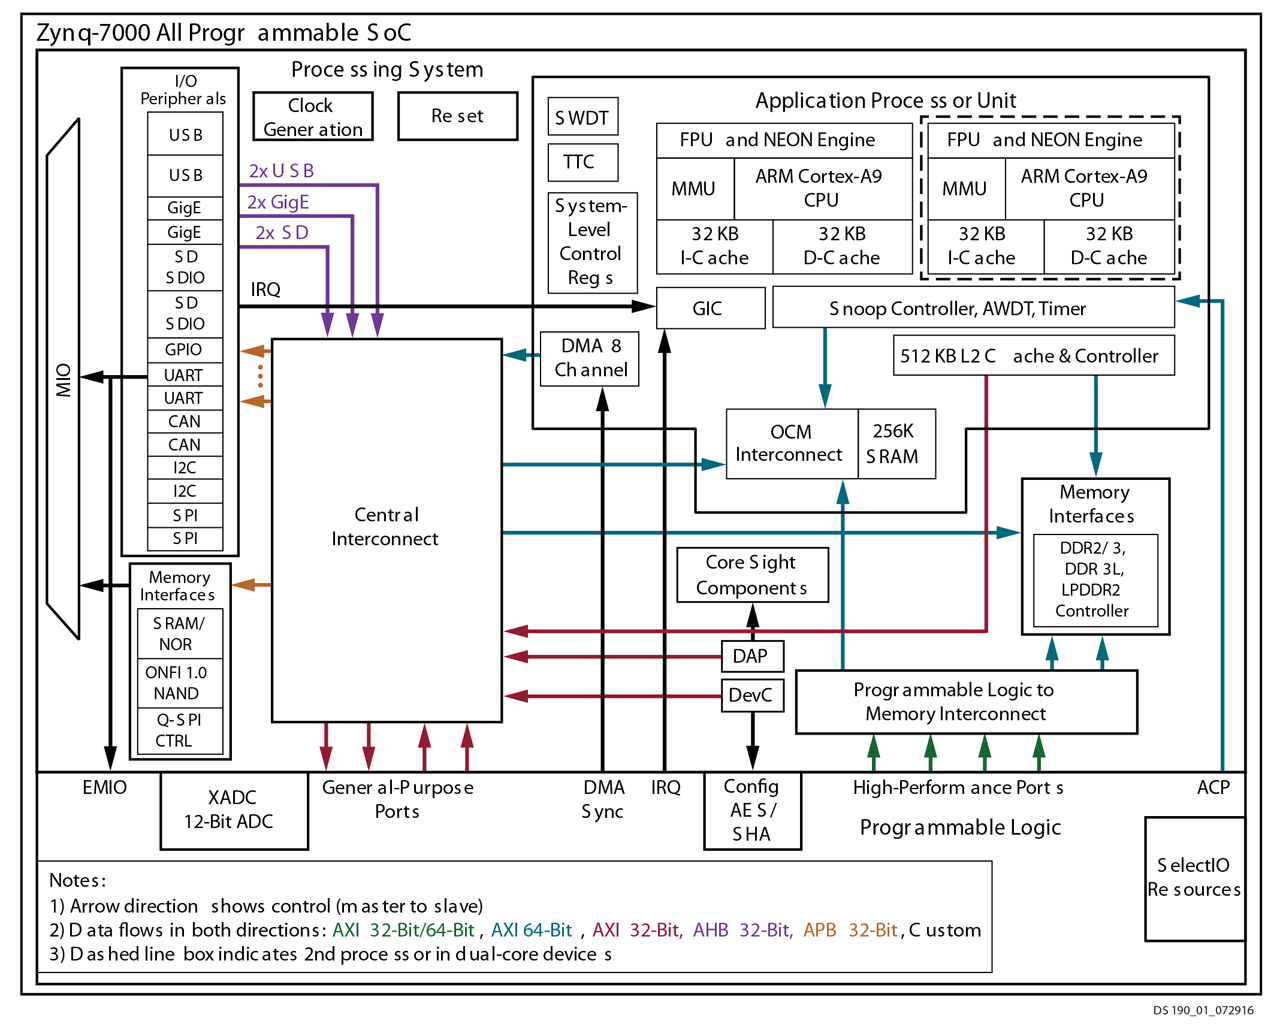
\includegraphics[width=1\textwidth]{images/Zynq-7000-Overview}
    \caption{Schemat ogólny architektury układu Zynq-7000.}
    \label{fig:zynq7000}
\end{figure}

\section{Interfejs AXI}
 AXI (ang. Advanced eXtensible Interface zawansowany rozszerzalny interfejs) jest częścią ARM AMBA (ang. Advanced Microcontroller Bus Architecture) – otwartego standardu, specyfikacją do zarządzania i połączeń między blokami funkcyjnymi w SoC. Aktualnie jest stosowana AMBA 4.0 która wprowadziła drugą wersję AXI, AXI4. Występują trzy typy interfejsów dla AXI4:
\begin{itemize}
\item AXI4 – stosowany w wysokowydajnych transferach w przestrzeni pamięci (ang. memory-mapped)
\item AXI4-Lite – stosowany dla prostszych operacji w przestrzeni pamięci (na przykład do komunikacji z rejestrami kontrolnymi i statusu)
\item AXI4-Stream – stosowany do wysokiej prędkości transmisji strumieniowych
\end{itemize}
Specyfikacja interfejsu zakłada komunikację pomiędzy pojedynczym AXI master i pojedynczym AXI slave, która ma na celu wymianę informacji pomiędzy tymi dwoma blokami funkcyjnymi IP core. Kilkanaście interfejsów AXI master i slave mogą zostać połączone między sobą za pomocą specjalnej struktury zwanej interconnect block (blok międzypołączeniowy) w której odbywa się trasowanie połączeń do poszczególnych bloków. 

AXI4 i AXI4-Lite składają się z 5 różnych kanałów:
\begin{itemize}
\item Kanał adresu odczytu,
\item Kanał adresu zapisu,
\item Kanał danych odczytanych
\item Kanał danych do zapisania
\item Kanał potwierdzenia zapisu
\end{itemize}
Dane mogą płynąć w obie strony pomiędzy master a slave jednocześnie. Ilość danych które można przesłać w jednej transakcji w przypadku AXI4 wynosi 256 transferów, zaś AXI4-Lite pozwala na tylko 1 transmisję.

AXI4-Stream nie posiada pola adresowego, a dane mogą być przesyłane nieprzerwanie. 
\subsection{Wykorzystanie AXI-Stream do transmisji sygnału video.} 
W odróżnieniu od klasycznej implementacji przetwarzania strumieniowego video, w AXI-Stream przesyłane są jedynie aktywne piksele. Linie synchronizacji poziomej i pionowej są odrzucane albo są połączane do specjalnego bloku detekcji timingów który mierzy parametry wchodzącego strumienia wizyjnego (ilość pikseli na linie, czas ilość aktywnych linii, czas wyciemnienia itd.). Podobnie informacje o synchronizacji są dodawane przez blok generujący timingi.

Do transmisji wykorzystane jest 6 linii: jedna linia danych i pięć kontrolno-sterujących. 
\begin{itemize}
\item Video Data – linia danych o szerokości jednego (albo dwóch) pikseli. Szerokość tej linii powinna być wielokrotnością liczby osim (16, 24, 48 itd.)
\item Valid – Linia podająca czy dane piksela są poprawne,
\item Ready – Linia kontrolna informująca urządzenie master że slave jest gotowy do transmisji danych,
\item Start Of Frame – linia która wskazuje pierwszy piksel nowej ramki,
\item End Of Line – linia wskazująca ostatni piksel w linii.
\end{itemize}
Aby mógł wystąpić poprawny transfer danych linie Valid i Ready muszą być w stanie wysokim podczas rosnącego zbocza zegara. Przykładowe nawiązanie transmisji przedstawia rysunek \ref{fig:handshake}

\begin{figure}[h]
    \centering
    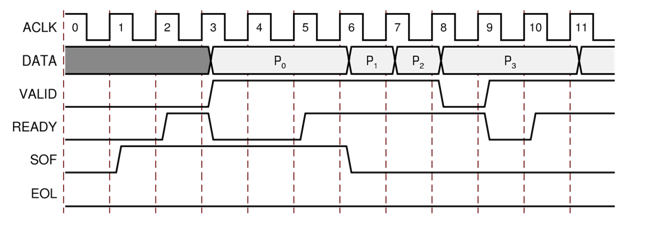
\includegraphics[width=1\textwidth]{images/axi-stream_hendshake}
    \caption{Przykład rozpoczęcia transmisji Reday/Valid.}
    \label{fig:handshake}
\end{figure}
Mając do dyspozycji układ heterogeniczny rodziny Zynq-7000 od firmy Xilinx operacje zostały podzielone między programowalną logiką a systemem procesorowym. Ogólny zarys systemu został przedstawiony na rysunku \ref{fig:systemwizyjny}.

\begin{figure}[h]
    \centering
    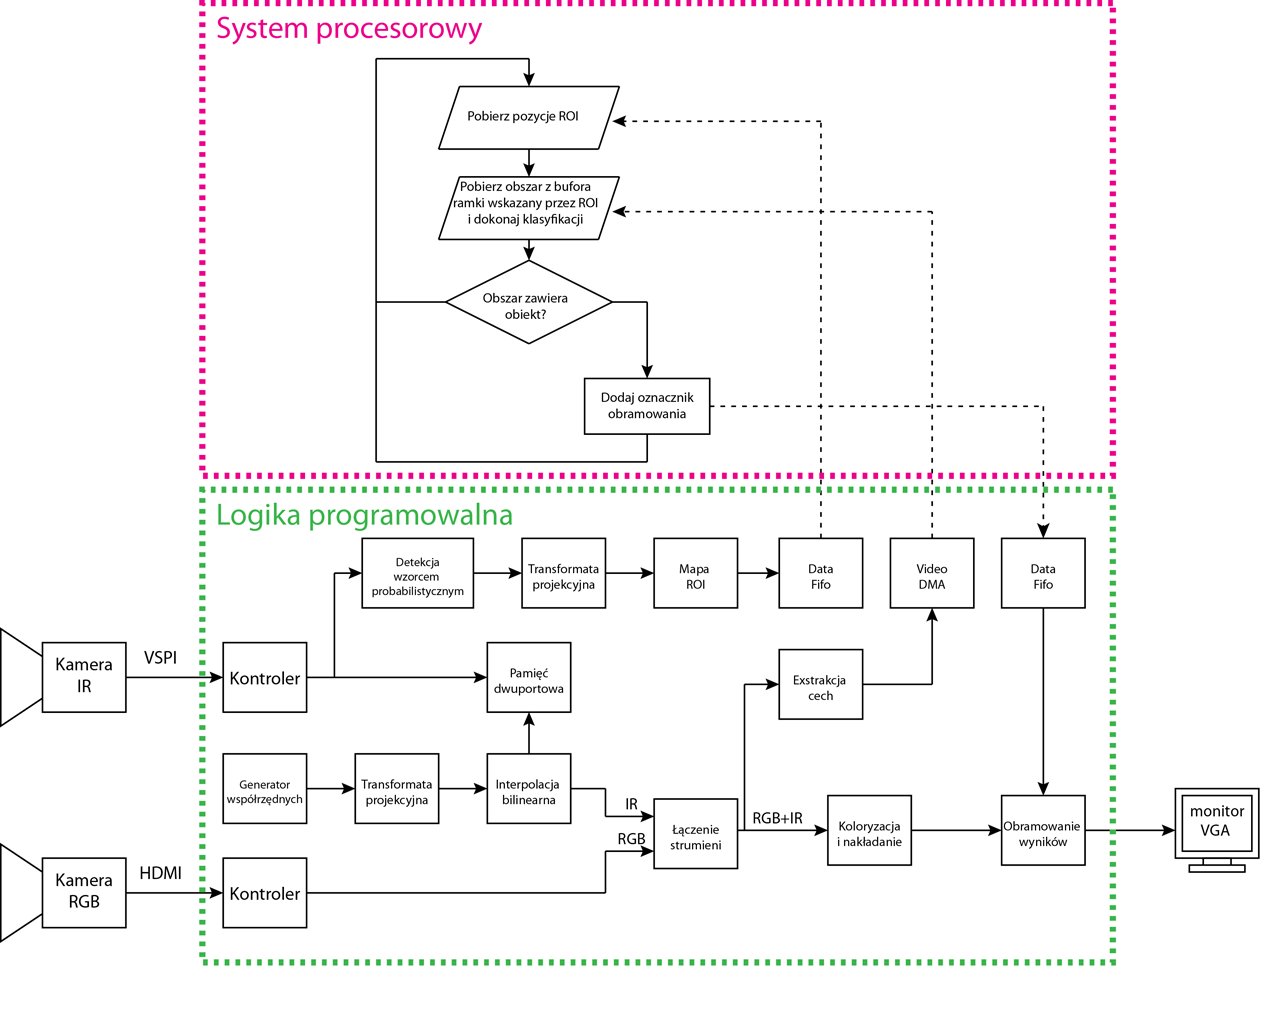
\includegraphics[width=1\textwidth]{images/system}
    \caption{Schemat blokowy systemu detekcji.}
    \label{fig:systemwizyjny}
\end{figure}

Programowalna logika:
\begin{itemize}
\item Akwizycja Obrazu poprzez HDMI (RGB) i VoSPI (IR),
\item Transformata projekcyjna i interpolacja obrazu IR,
\item Nałożenie i synchronizacja obrazu IR do obrazu RGB,
\item Ekstrakcja cech z połączonych obrazów,
\item Prezentacja wyników,
\item Detekcja kandydatów za pomocą wzorca probabilistycznego.
\end{itemize}
System Procesorowy:
\begin{itemize}
\item konfiguracja parametrów systemu wizyjnego w logice programowalnej poprzez interfejs AXI-Lite,
\item Klasyfikacja obszarów wytypowanych przez wzorzec probabilistyczny,
\item Generowanie oznaczników.
\end{itemize}

\section{Opis modułów}

\subsection{Transformata projekcyjna}
Zadaniem modułu jest dostosowanie obrazu IR by pokrywał się z obrazem RGB. Moduł transformaty projekcyjnej zamienia wygenerowane współrzędne w zakresie wielkości przychodzącego obrazu RGB na odpowiadające im punkt na obrazie IR (wraz z częścią ułamkową). Moduł jest konfigurowalny poprzez interfejs AXI-Lite, za pomocą którego można ustawić wartość minimalną i maksymalną współrzędnych wyjściowych U i V oraz macierz transformaty.
\subsection{Kontroler kamery IR}
Pobiera obraz z kamery poprzez interfejs VoSPI który następnie zostaje zapisany do dwuportowej pamięci BRAM.
\subsection{Interpolacja bilinearna}
Prosty moduł przeznaczony głównie do powiększania obrazów. Pobiera wartość 4 otaczających, podanych na wejściu punktu, pikseli z BRAM i na ich bazie jest wykonywana interpolacja. Moduł zapamiętuje 4 ostatnio użyte piksele które są na bieżąco aktualizowane wraz z zmianą położenia punktu wejściowego na obrazie IR.
\subsection{Łączenie strumieni}
Moduł posiada dwa wejścia dla obrazu. Jeden strumień jest głównym i do niego jest dołączany drugi strumień. Do synchronizacja strumieni została wykorzystana możliwość AXI-Strem do wstrzymania transmisji. Piksele z dołączanego strumienia są odrzucane do momentu pojawienia się sygnału SOF. W momencie pojawienia się sygnału SOF w strumieniu głównym transmisja zostaje wznowiona pod kontrolą strumienia wyjściowego. 
\subsection{Koloryzacja i nakładanie}
Połączone strumienie RGB+IR zostają połączone w jeden obraz. Obraz IR zostaje poddany koloryzacji na podstawie 12-bitowego LUT i nałożony w proporcjach 50 na 50 z obrazem RGB.
